%----------------------------------------------------------------------------
\chapter{\bevezetes}
%----------------------------------------------------------------------------

A bevezető tartalmazza a diplomaterv-kiírás elemzését, történelmi előzményeit, a feladat indokoltságát (a motiváció leírását), az eddigi megoldásokat, és ennek tükrében a hallgató megoldásának összefoglalását.

A bevezető szokás szerint a diplomaterv felépítésével záródik, azaz annak rövid leírásával, hogy melyik fejezet mivel foglalkozik.

\begin{figure}[htbp]
  \centering
  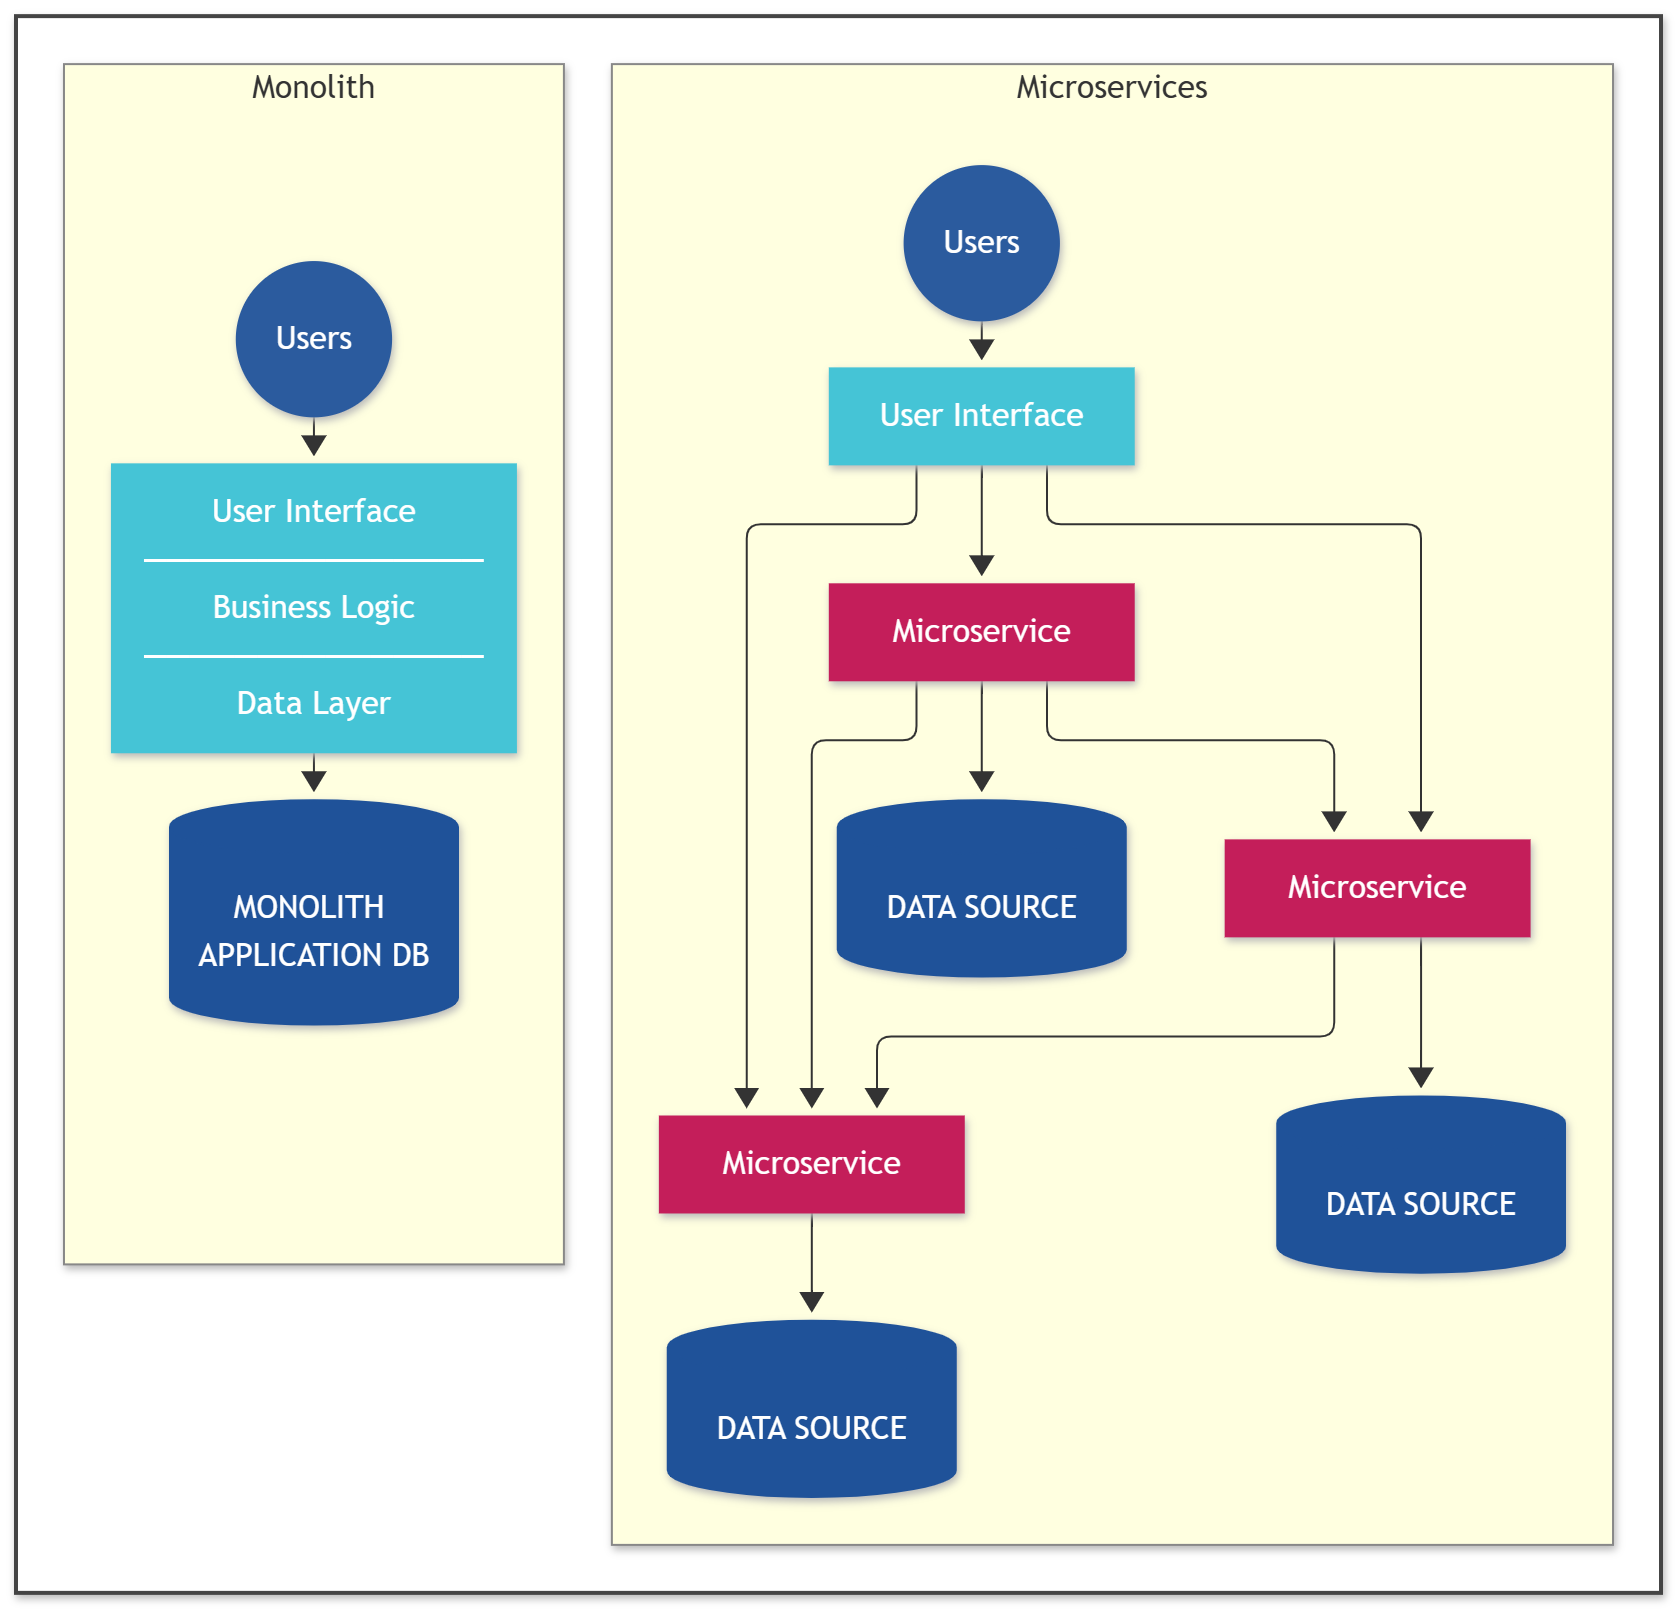
\includegraphics[width=0.7\textwidth]{figures/mermaid-cloud_vs_monolith.png}
  \caption{Cloud vs Monolith Architecture}
  \label{fig:cloud-vs-monolith}
\end{figure}